\documentclass[a4paper,12pt]{ctexart}
\usepackage[margin=2cm]{geometry}
\usepackage{graphicx}
\usepackage{subfigure}
\usepackage{float}
\usepackage[colorlinks,linkcolor=black]{hyperref}%colorlinks启用链接颜色,linkcolor指定对应的颜色
\pagestyle{empty}
\begin{document}

\begin{center}
\huge \textbf{Design Ubuntu}
\end{center}

\tableofcontents

\newpage
\section{安装新的主题}
\subsection{Numix主题}
Ubuntu用户安装PPA,打开终端,输入命令(支持Ubuntu13.10,13.04和12.10):
\begin{verbatim}
sudo add-apt-repository ppa:satyajit-happy/themes
sudo apt-get update
sudo apt-get install numix-gtk-theme
\end{verbatim}
Numix的界面大致如下:
\begin{figure}[H]
  \centering
  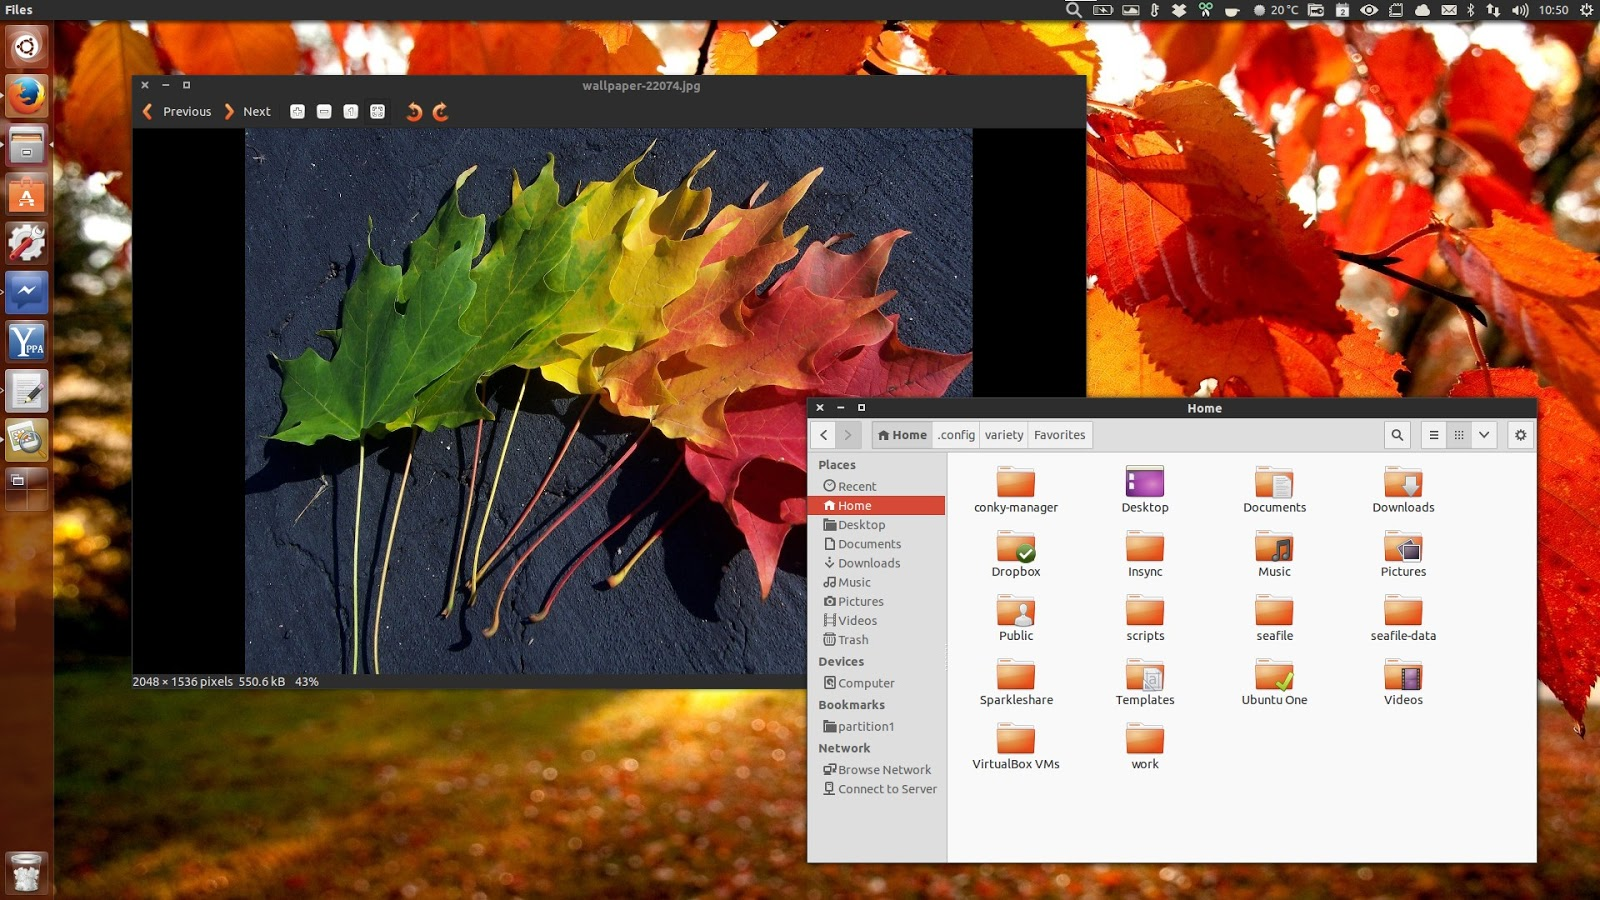
\includegraphics[width=10cm]{Figures/Numix_theme_1.jpg}
\end{figure}

\begin{figure}[H]
  \centering
  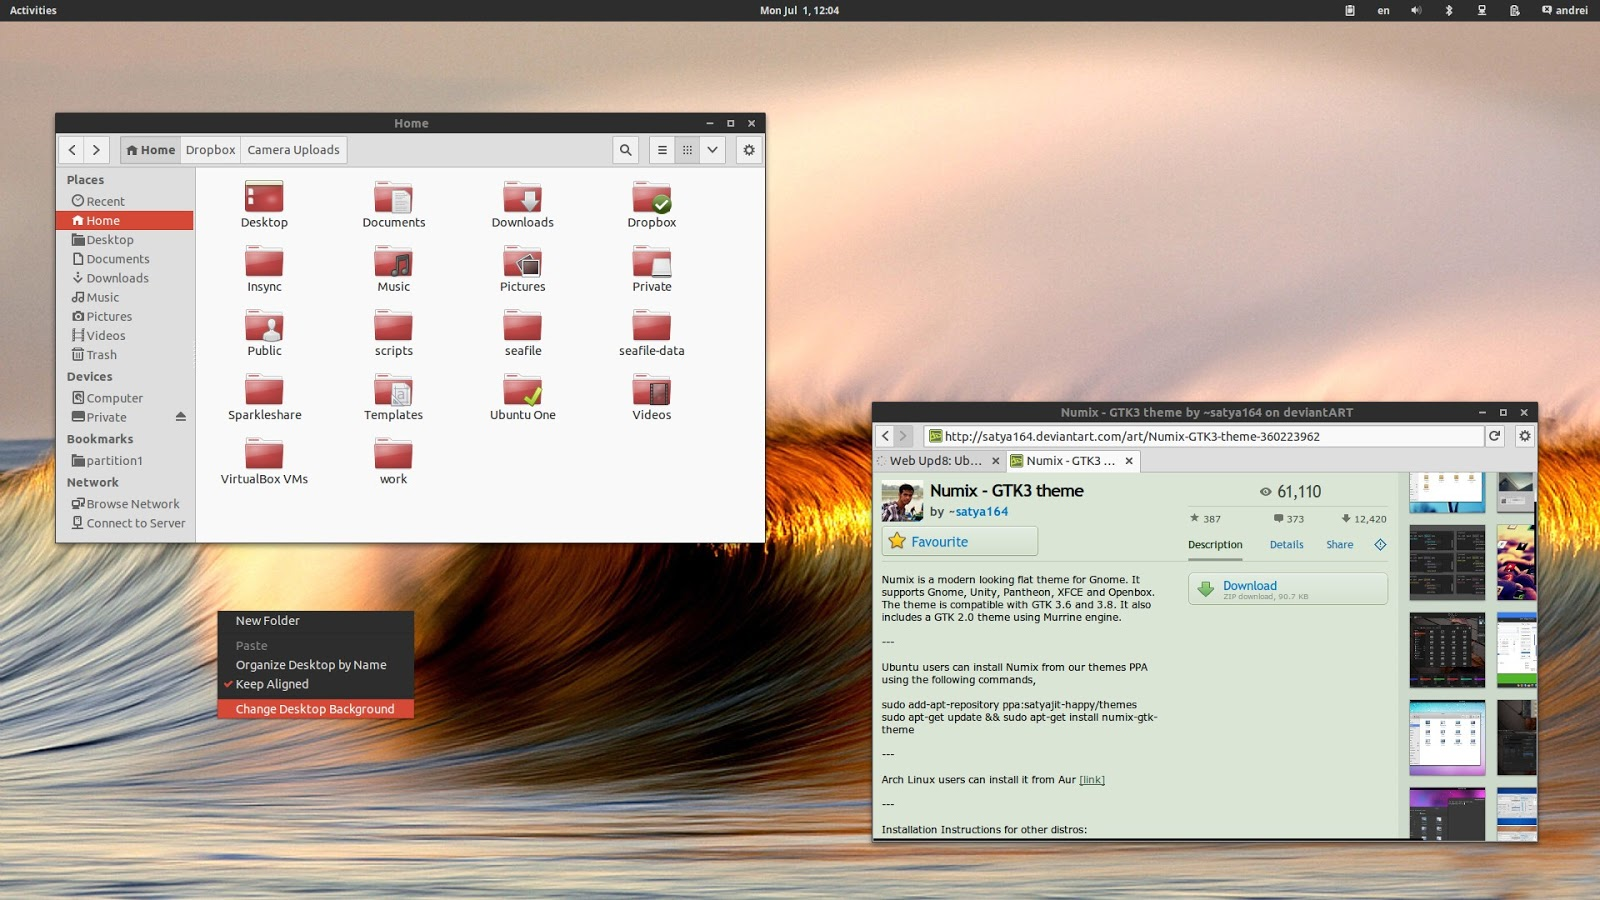
\includegraphics[width=10cm]{Figures/Numix_theme_2.jpg}
\end{figure}


\newpage
\section{动态壁纸}
下载安装LiveWallPaper,命令如下,三个相关的软件都要安装。
\begin{verbatim}
sudo add-apt-repository ppa:fyrmir/livewallpaper-daily
sudo apt-get update
sudo apt-get install livewallpaper
sudo apt-get install livewallpaper-config livewallpaper-indicator
\end{verbatim}



\newpage
\section{调整启动器的位置}
有两种方法可以调整启动器的位置。
\subsection{在终端输入命令}
\begin{verbatim}
gsettings set com.canonical.Unity.Launcher launcher-position Bottom
\end{verbatim}
\subsection{在unity-tweak-tool中设置}
其原理和输入命令是一样的。
\newpage
\section{设置终端的颜色和字体}
打开终端右击选择Profiles$\rightarrow$Colors$\rightarrow$Text and Background Color$\rightarrow$Built-in schemes$\rightarrow$Green on black。

打开终端右击选择Profiles$\rightarrow$General$\rightarrow$Text Appearance$\rightarrow$Custom font$\rightarrow$AR PL UKai CN Bold。
\end{document}
